%-------------
% Resultados e Discussão
%--------------------------
\chapter{Resultados e Discussão} \label{Resultados e Discussão}

Este capítulo apresenta os resultados obtidos ao longo do trabalho, abrangendo uma breve análise da dispersão da base de dados experimental, o desempenho dos modelos de classificação e regressão desenvolvidos e a validação experimental do sistema proposto em tempo real.

% ---------------------------------------------------------------------------
\section{Base experimental coletada}
A Figura \ref{fig:dispersao_potencia_corrente} apresenta um gráfico de dispersão entre corrente elétrica e potência ativa para as amostras coletadas. Observa-se a formação de agrupamentos distintos de pontos associados aos diferentes tipos de carga, indicando que essas grandezas apresentam padrões característicos para cada configuração analisada.

Esse comportamento evidencia que as variáveis elétricas medidas possuem forte capacidade discriminativa, o que favorece o processo de aprendizado do modelo de classificação. Dessa forma, os dados experimentais apresentam separabilidade significativa no espaço de características, contribuindo para o elevado desempenho obtido pelos modelos de aprendizado de máquina. O código desenvolvido dessa análise está disponível no Apêndice \ref{apendice_análise_PZEM}.

\begin{figure}[!htbp]
    \centering
    \caption{Gráfico de dispersão entre corrente e potência ativa das amostras coletadas.}
    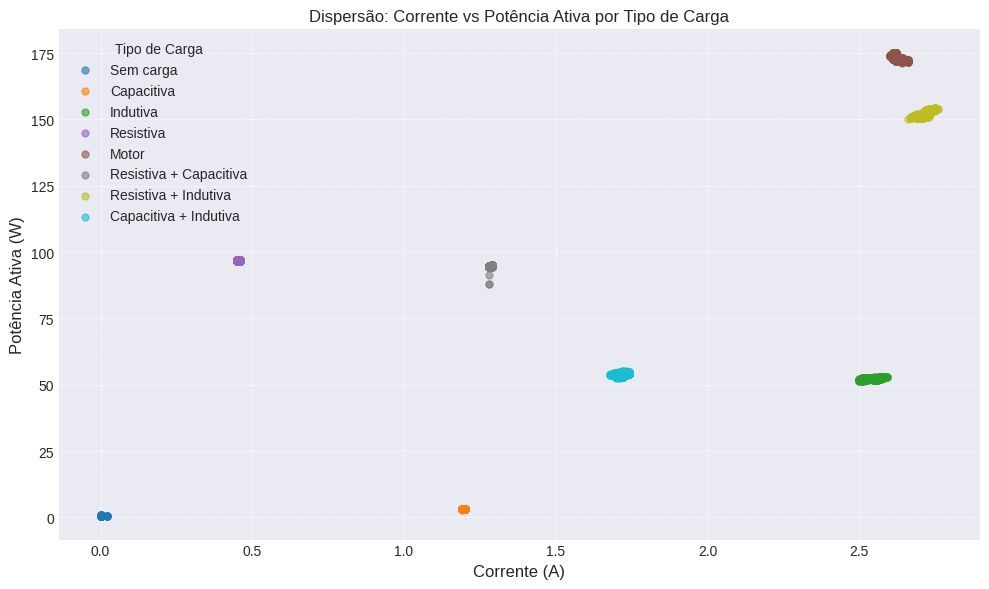
\includegraphics[width=1\textwidth]{Figuras/grafico de dispersao I vs P por tipo de carga.png}
    \fonte{\me{2026}}
    \label{fig:dispersao_potencia_corrente}
\end{figure}

% ---------------------------------------------------------------------------
\section{Desempenho do modelo de classificação}
O desempenho do modelo de classificação foi avaliado por meio das métricas de acurácia, precisão, \textit{recall} e \textit{F1-score}, além da análise da matriz de confusão obtida no conjunto de teste. O treinamento foi conduzido por 40 épocas, com monitoramento da perda (\textit{loss}) e acurácia tanto para os conjuntos de treinamento quanto de validação.

Observa-se que o modelo atingiu acurácia de 100\% no treinamento a partir da época 29, com valores de perda próximos de zero (\textit{val\_loss} de 0,0048 ao final do treinamento). Os resultados de precisão, recall e F1-score foram iguais a 1,0 para todas as classes avaliadas, indicando que o erro do modelo foi praticamente nulo (inferior a 0,5\% ao final das 40 épocas). A Figura \ref{fig:graficos_modelo_classificacao} apresenta a evolução da acurácia e da perda ao longo das épocas de treinamento. 

A matriz de confusão apresentada na Figura \ref{fig:matriz_confusao} demonstra que todas as amostras foram corretamente classificadas pelo modelo, sem ocorrência de erros entre as categorias de carga. A diagonal principal da matriz apresenta valores máximos para todas as classes, confirmando a eficácia do modelo em distinguir os diferentes tipos de carga analisados.

\begin{figure}[!htbp]
    \centering
    \caption{Matriz de confusão do modelo de classificação de cargas.}
    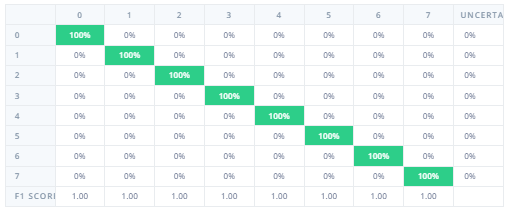
\includegraphics[width=\textwidth]{Figuras/matriz de confusao modelo de classificacao.png}
    \fonte{\me{2026}}
    \label{fig:matriz_confusao}
\end{figure}

Esses resultados evidenciam que as variáveis elétricas utilizadas como entrada apresentam forte capacidade de distinção entre os diferentes tipos de carga analisados. Além disso, a separabilidade observada nos dados experimentais, conforme demonstrado na Figura \ref{fig:dispersao_potencia_corrente}, contribuiu significativamente para facilitar o processo de aprendizado da rede neural, permitindo que o modelo convergisse rapidamente para uma solução ótima.

\begin{figure}[h]
    \centering
    \caption{Métricas de desempenho do modelo de classificação ao longo das épocas de treinamento.}
    \subfigure[Evolução da acurácia.]{
        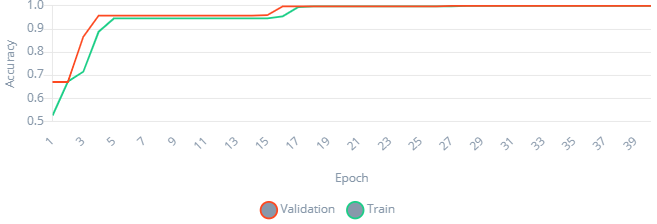
\includegraphics[width=0.9\textwidth]{Figuras/grafico de acuracia modelo classificacao.png}
    }
    \hfill
    \subfigure[Evolução da perda (loss).]{
        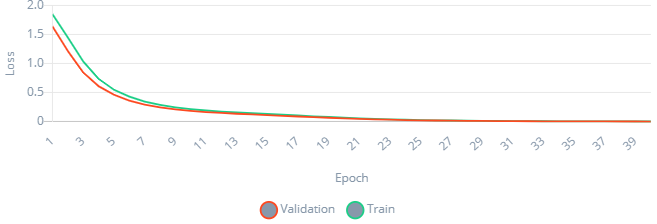
\includegraphics[width=0.9\textwidth]{Figuras/grafico de erro modelo de classificacao.png}
    }
    \hfill
    \subfigure[Evolução do treinamento do modelo.]{
        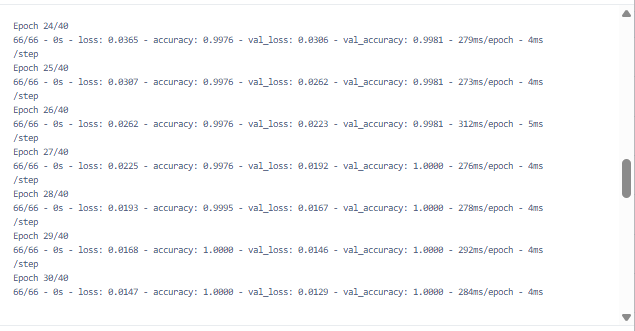
\includegraphics[width=0.9\textwidth]{Figuras/treinamento modelo classificao.png}
    }
    \fonte{\me{2026}} 
    \label{fig:graficos_modelo_classificacao}
\end{figure}

% ---------------------------------------------------------------------------
\section{Desempenho do modelo de regressão}
O desempenho do modelo de regressão foi avaliado utilizando as métricas de erro quadrático médio (MSE) e erro absoluto médio (MAE), além da análise da evolução da perda durante o treinamento. A Figura \ref{fig:graficos_modelo_regressao} apresenta a evolução do erro ao longo das épocas de treinamento. Observa-se que o modelo convergiu rapidamente, atingindo valores de perda próximos de zero já nas primeiras épocas. Ao final do treinamento, os valores de perda estabilizaram-se em torno de $0,94967 \times 10^{-5}$ para o treinamento e $3,3 \times 10^{-5}$ para a validação.

\begin{figure}[h]
    \centering
    \caption{Métricas de desempenho do modelo de regressão ao longo das épocas de treinamento.}
    \subfigure[Evolução da perda (loss).]{
        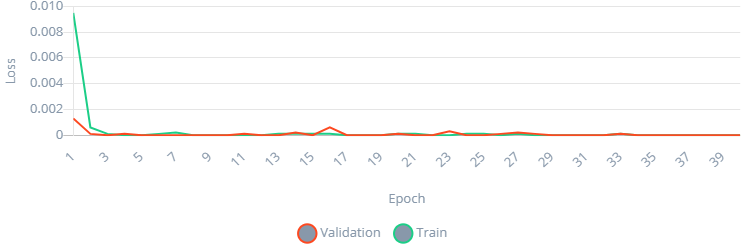
\includegraphics[width=0.9\textwidth]{Figuras/grafico de erro modelo de regressao.png}
    }
    \hfill
    \subfigure[Evolução do treinamento do modelo.]{
        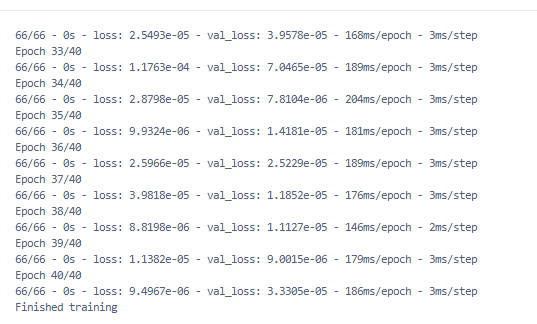
\includegraphics[width=0.7\textwidth]{Figuras/treinamento modelo regressão.png}
    }
    \fonte{\me{2026}}
    \label{fig:graficos_modelo_regressao}
\end{figure}


No conjunto de teste, o modelo apresentou MSE de $8,3 \times 10^{-6}$ e MAE de 0,00228, indicando elevada precisão na estimação do fator de potência. O coeficiente de variância explicada (\textit{explained variance score}) atingiu 0,9997, demonstrando que o modelo é capaz de explicar 99,97\% da variância dos dados, o que evidencia um excelente ajuste.

A Tabela \ref{tab:metricas_regressao} resume as principais métricas de desempenho obtidas pelo modelo nos conjuntos de validação e teste.

\begin{table}[h]
    \centering
    \caption{Métricas de desempenho do modelo de regressão.}
    \label{tab:metricas_regressao}
    \begin{tabular}{lccc}
    \hline
    \textbf{Conjunto} & \textbf{MSE} & \textbf{MAE} & \textbf{Variância Explicada} \\
    \hline
    Validação (float32) & $7,81 \times 10^{-6}$ & 0,00224 & 0,99972 \\
    Teste (float32) & $8,30 \times 10^{-6}$ & 0,00228 & 0,99970 \\
    \hline
    \end{tabular}
    \fonte{\me{2026}}
\end{table}

Os resultados obtidos demonstram que o modelo de regressão é capaz de estimar o fator de potência com erro extremamente baixo, sendo que essa precisão é atribuída principalmente à qualidade dos dados experimentais.

% ---------------------------------------------------------------------------
\section{Validação do sistema em tempo real}
% O sistema foi implementado em bancada experimental, integrando sensor PZEM-004T, microcontrolador NodeMCU ESP8266, relés, contatores, medidor de referência e as seguintes cargas: lâmpada, transformador, três capacitores de 5 $\mu$F em paralelo e motor de indução. A Figura \ref{fig:sistema_montado} ilustra a configuração utilizada nos testes.

O sistema foi implementado em bancada experimental, integrando sensor PZEM-004T, microcontrolador NodeMCU ESP8266, Arduino Uno, módulos relé, contatores, medidor de referência e as seguintes cargas: lâmpada (carga resistiva), transformador (carga indutiva), três capacitores de 5 $\mu$F em paralelo (carga capacitiva) e motor de indução. A Figura \ref{fig:sistema_montado} ilustra a configuração utilizada nos testes.

A Figura \ref{fig:sistema_montado}(a) apresenta o sistema de cargas, composto pelos contatores, medidor de referência e os elementos de carga utilizados nos experimentos. Já a Figura \ref{fig:sistema_montado}(b) mostra o sistema de aquisição, transmissão e controle, destacando o sensor PZEM-004T, o microcontrolador NodeMCU ESP8266, o Arduino Uno utilizado no controle dos relés e os módulos relé responsáveis pelo acionamento das cargas.

\begin{figure}[h]
    \centering
    \caption{Sistema experimental desenvolvido para aquisição e monitoramento das grandezas elétricas.}
    \subfigure[Sistema de cargas.]{
        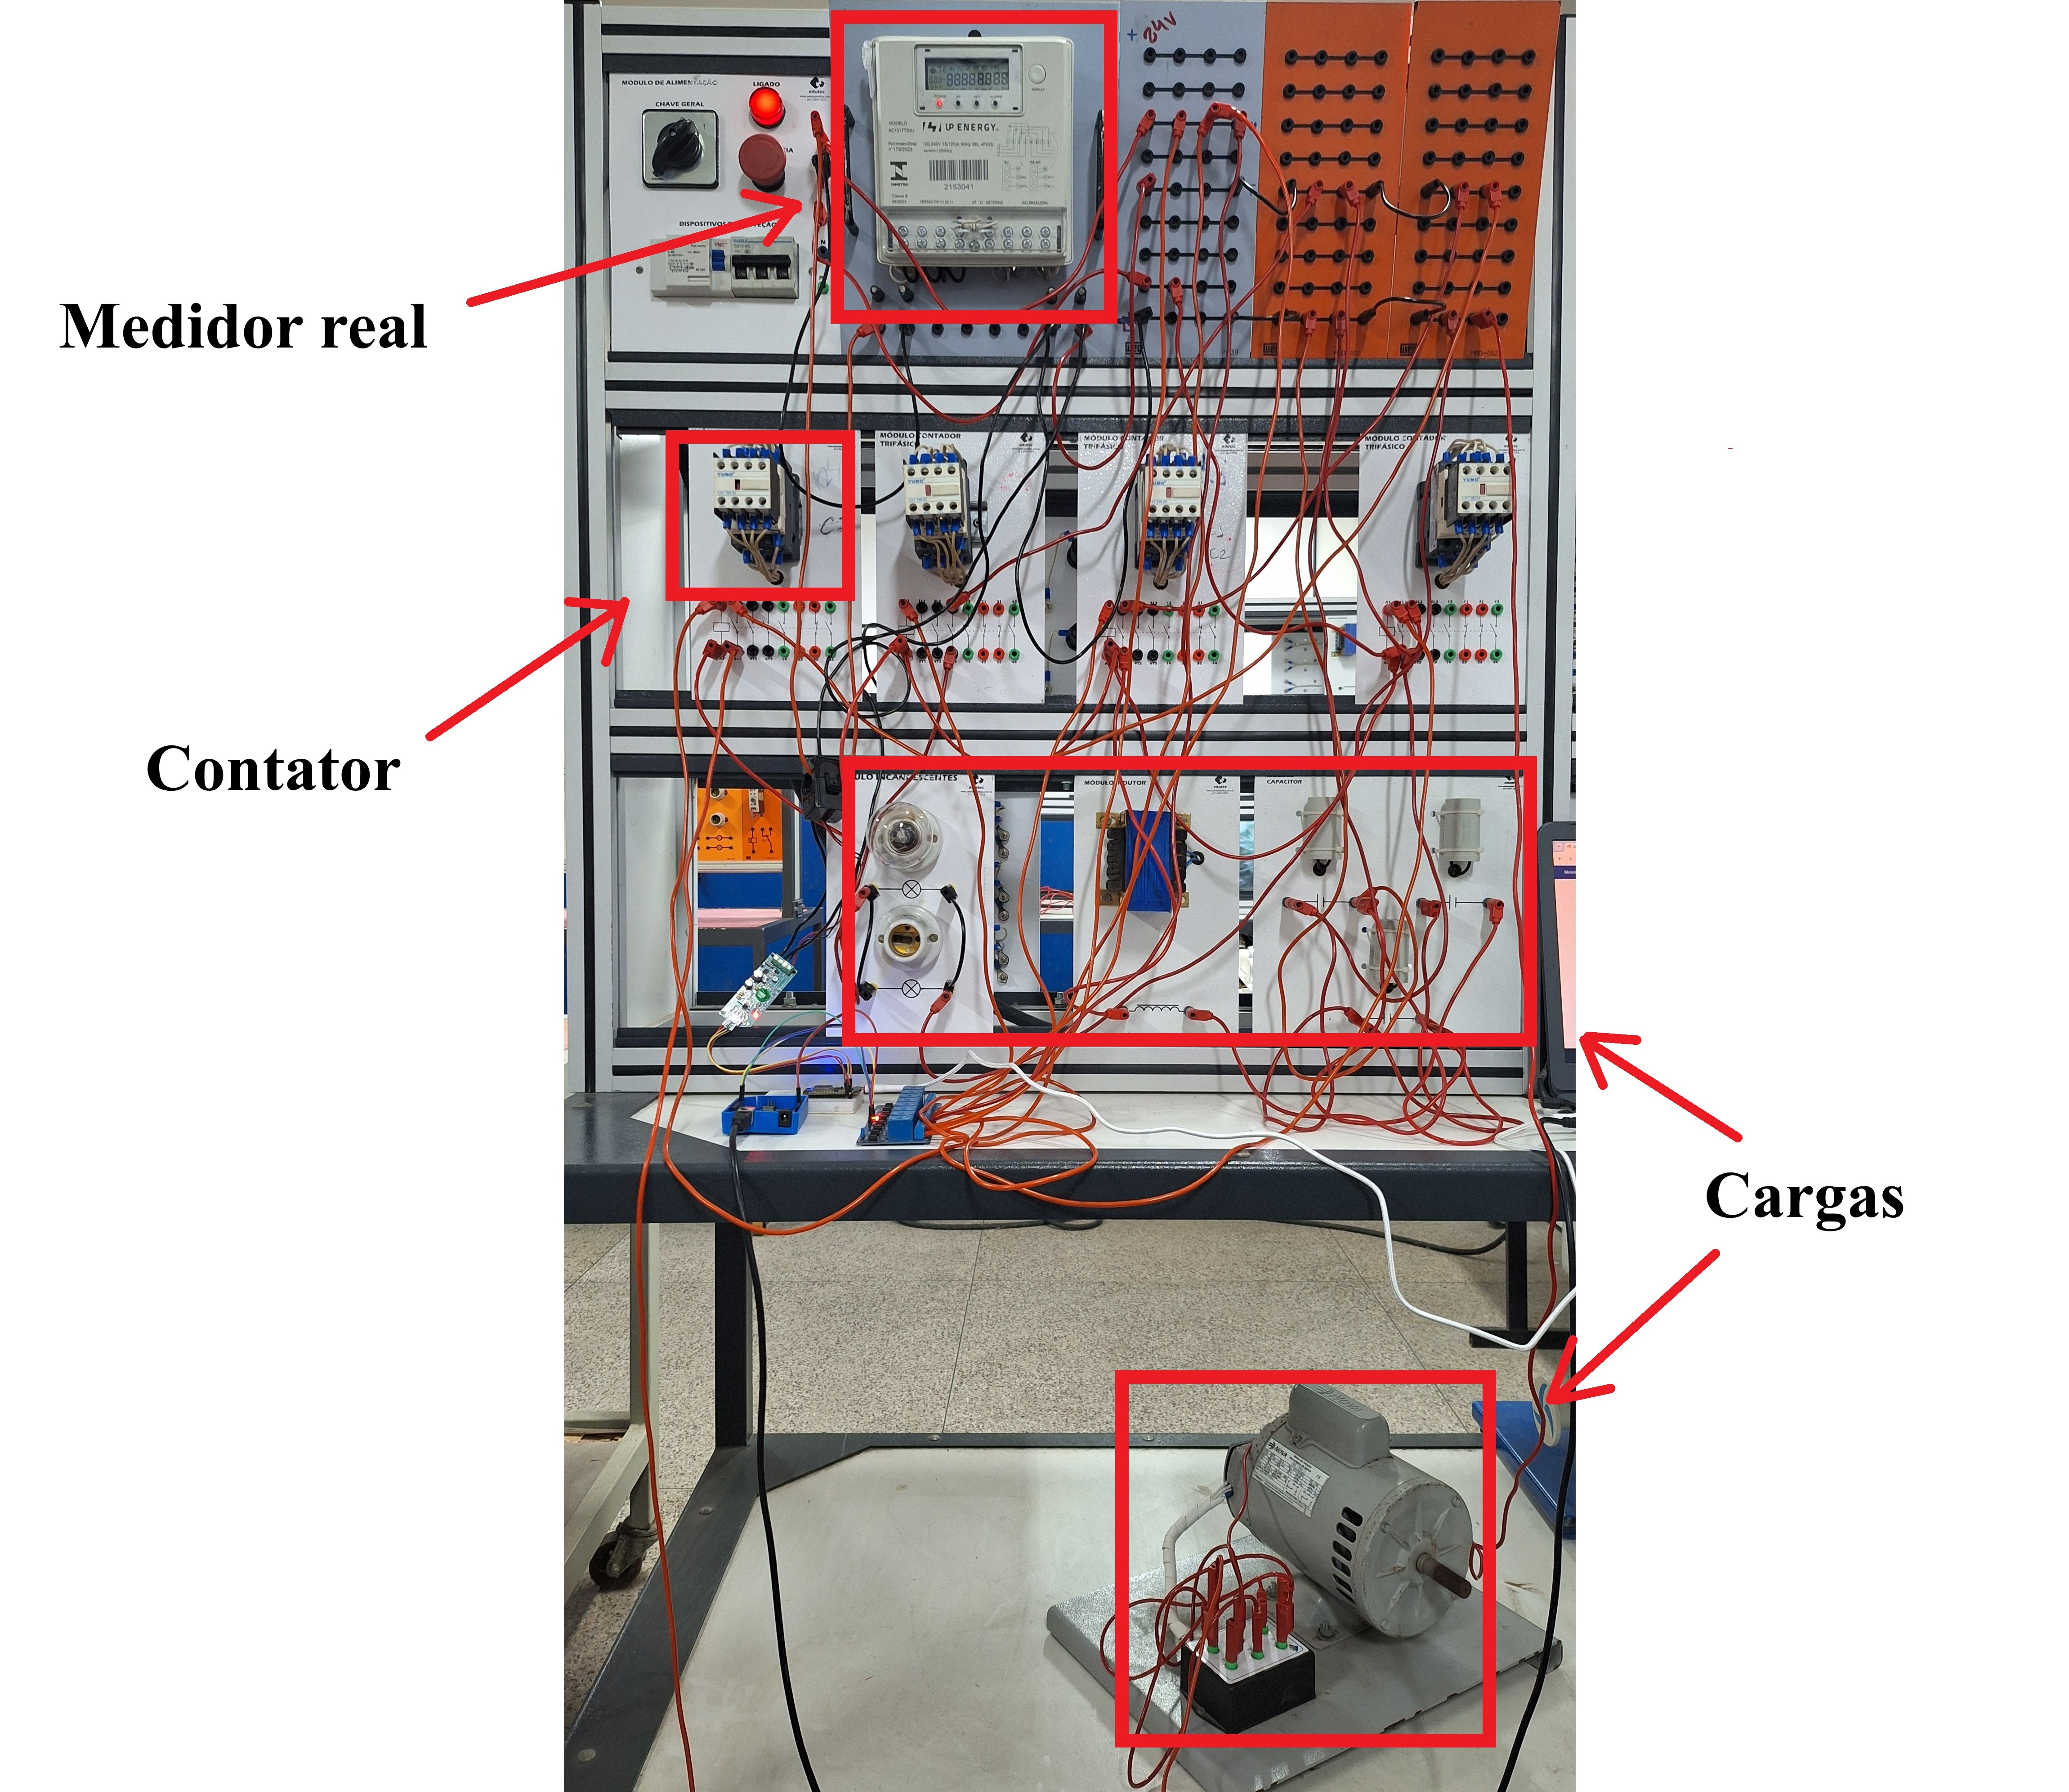
\includegraphics[width=0.8\textwidth]{Figuras/Sistema-montado.jpg}
    }
    \hfill
    \subfigure[Sistema de aquisição, transmissão e controle.]{
        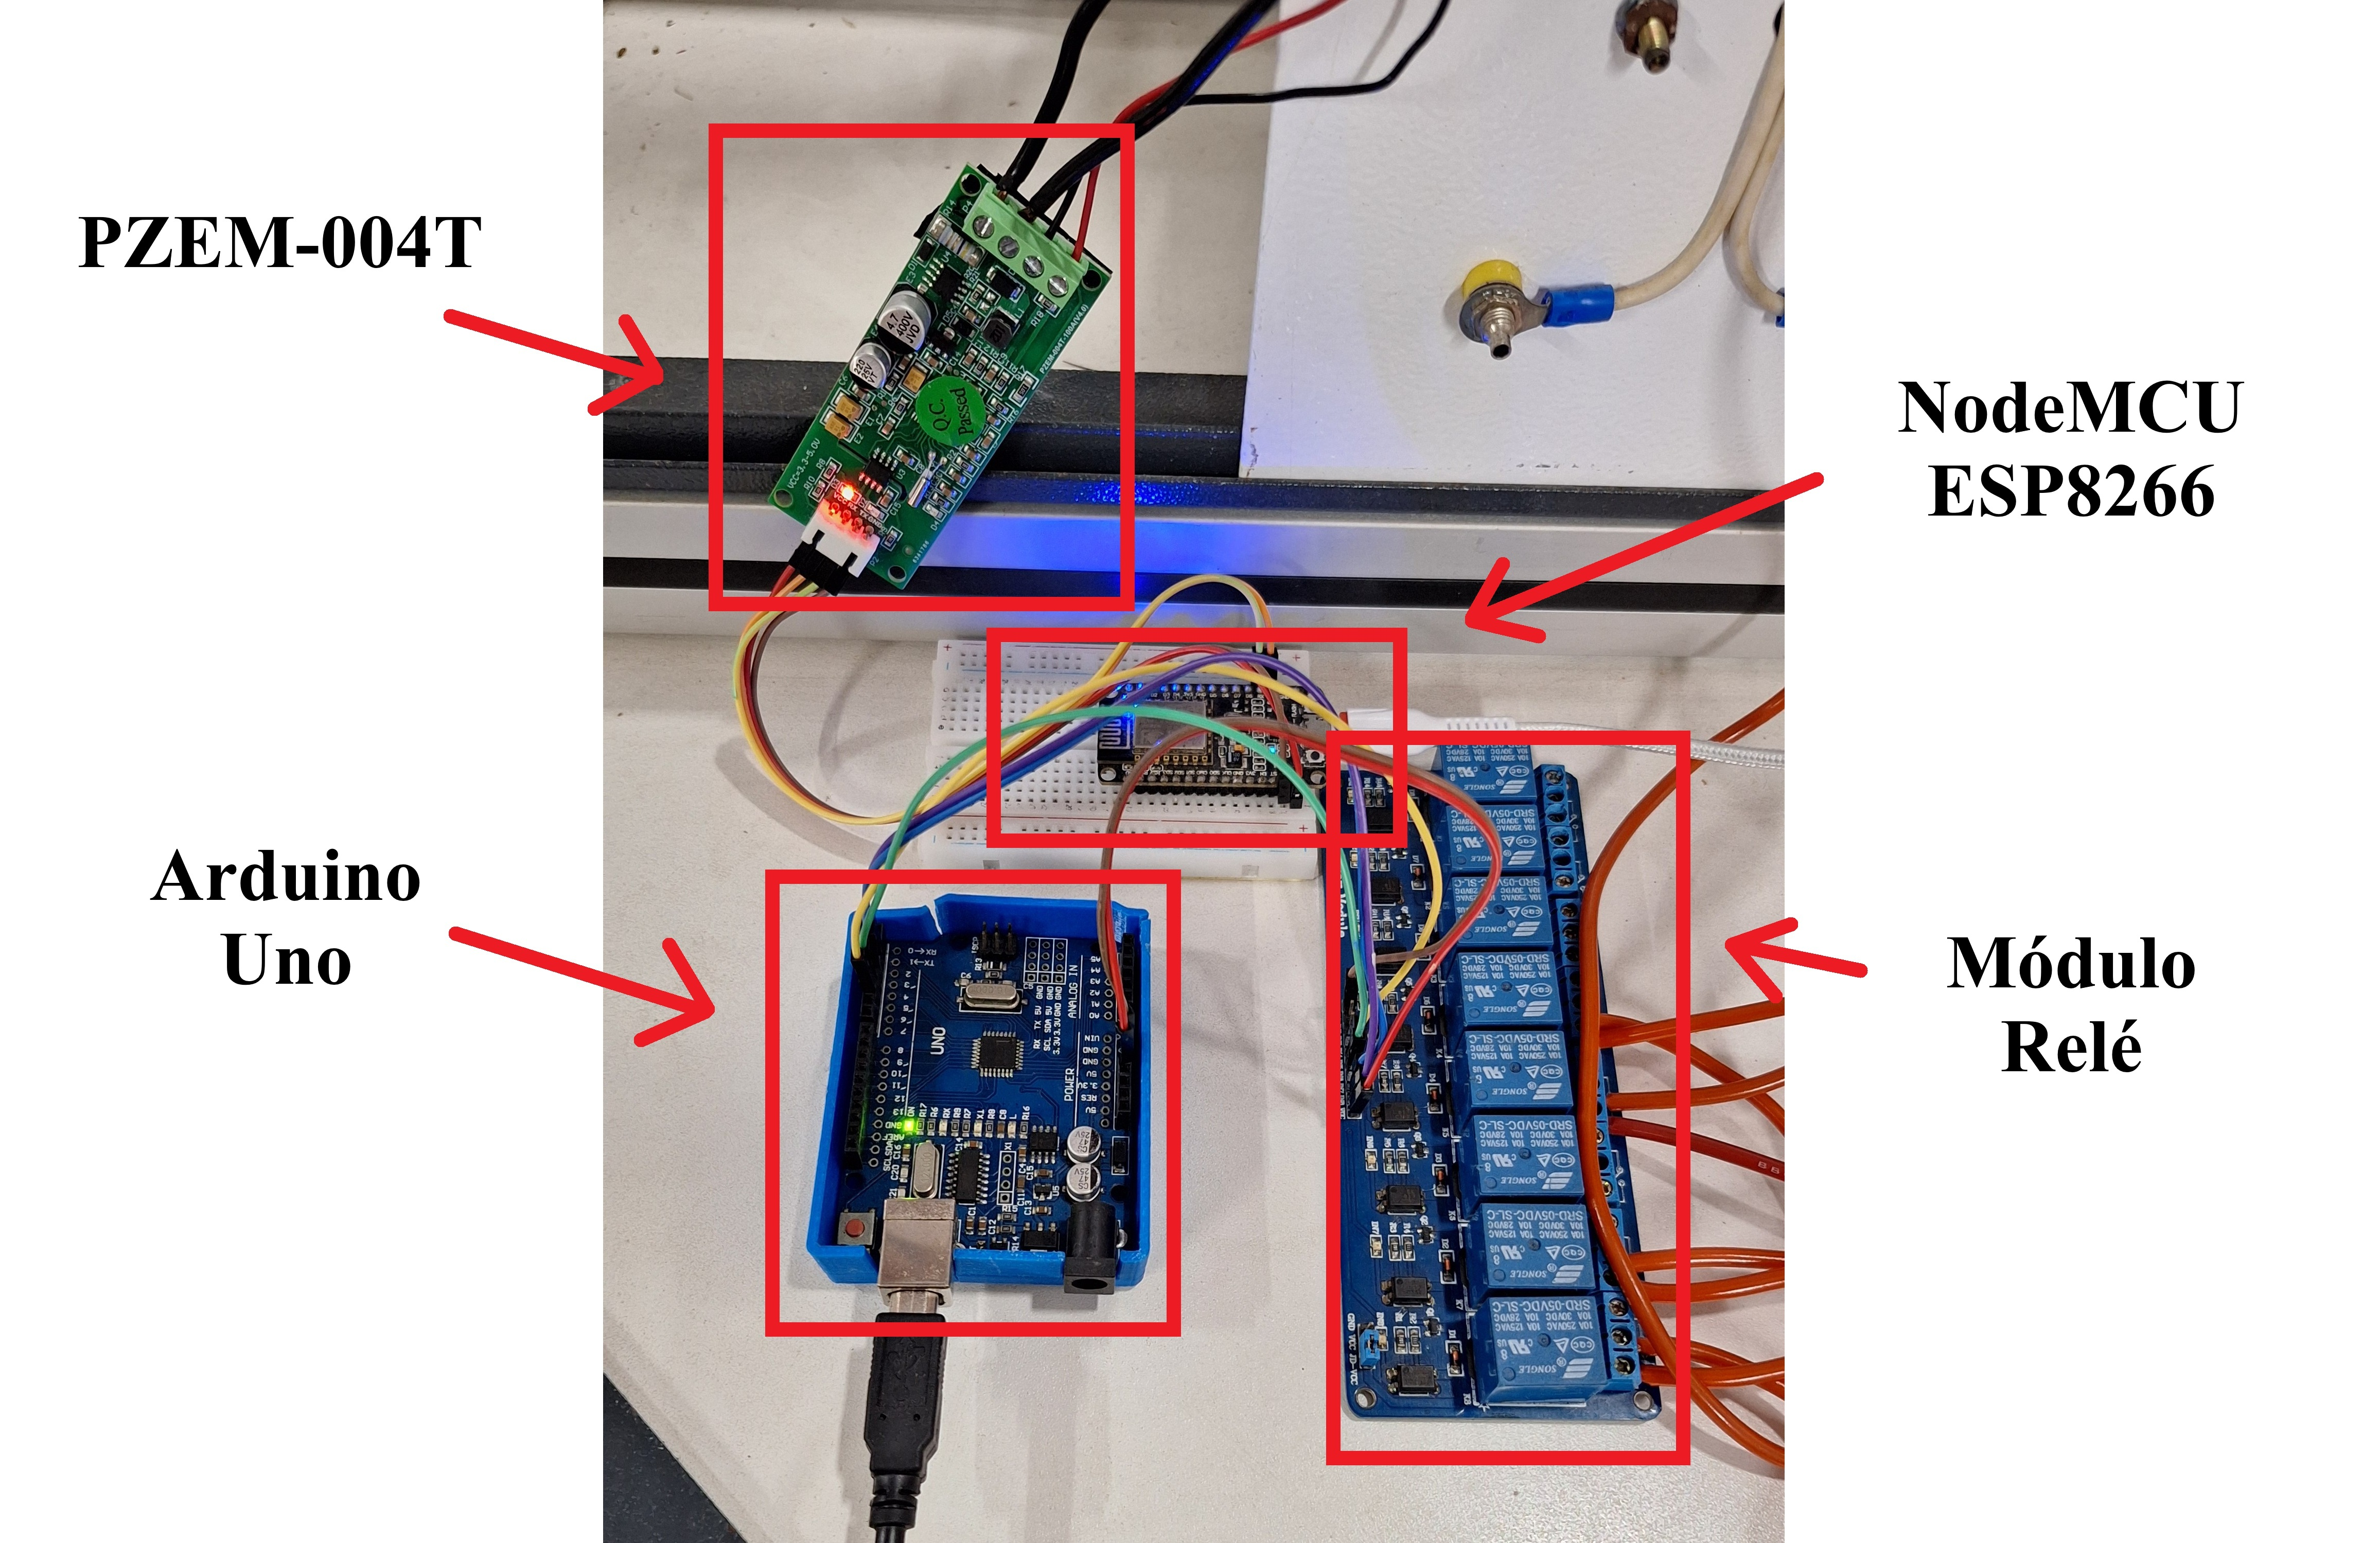
\includegraphics[width=0.7\textwidth]{Figuras/Sistema-pzem-rele-nodemcu.jpg}
    }
    \fonte{\me{2026}}
    \label{fig:sistema_montado}
\end{figure}

Durante os ensaios, as grandezas elétricas foram medidas pelo sensor PZEM-004T e transmitidas em tempo real ao Node-RED, onde foram processadas pelos modelos de aprendizado de máquina. Para validação, as medições do sensor e as estimativas dos modelos foram comparadas com um medidor comercial de referência. 

\begin{table}[!htbp]
    \centering
    \caption{Comparação entre medições do medidor de referência, sensor PZEM-004T e estimativas do modelo.}
    \begin{tabular*}{\textwidth}{@{\extracolsep{\fill}}lccccc@{}}
    \hline
    \textbf{Carga} & \textbf{FP (Ref.)} & \textbf{I (Ref.)} & \textbf{FP (PZEM)} & \textbf{I (PZEM)} & \textbf{FP Est.} \\
    \hline
    Sem carga & 1,00 & 0,00 & 1,00 & 0,00 & 0,29 \\
    Capacitiva & 0,00 & 1,19 & 0,01 & 1,23 & 0,02  \\
    Indutiva & 0,08 & 2,69 & 0,09 & 2,93 & 0,11  \\
    Resistiva & 1,00 & 0,45 & 1,00 & 0,46 & 1,01 \\
    Motor & 0,29 & 2,84 & 0,31 & 2,82 & 0,31 \\
    Resistiva + capacitiva & 0,36 & 1,29 & 0,34 & 1,32 & 0,34 \\
    Resistiva + indutiva & 0,25 & 2,75 & 0,25 & 2,96 & 0,25 \\
    Capacitiva + indutiva & 0,15 & 1,52 & 0,13 & 1,95 & 0,13 \\
    \hline
    \end{tabular*}
    \fonte{\me{2026}}
    \label{tab:validacao_tempo_real}
\end{table}

Conforme Tabela \ref{tab:validacao_tempo_real}, observam-se pequenas diferenças entre as leituras do medidor de referência e aquelas obtidas pelo sensor PZEM. Essas variações podem ser atribuídas à precisão limitada do sensor utilizado e às diferenças de resolução entre os equipamentos de medição, ou ainda, estarem associadas a possíveis imprecisões de calibração do sensor ou a pequenas resistências internas do dispositivo, como por exemplo na situação sem carga, em que o FP estimado foi de 0,29. Ainda assim, os resultados evidenciam que o modelo de regressão foi capaz de reproduzir adequadamente o comportamento das grandezas elétricas do sistema, mesmo diante de pequenas variações nas medições experimentais.

Além disso, o modelo de classificação foi capaz de identificar corretamente o tipo de carga em todos os cenários avaliados, demonstrando a viabilidade do sistema proposto para aplicações de monitoramento inteligente em tempo real.

% \newpage
Os resultados para cada cenário de carga podem ser observados nas Figuras \ref{fig:painel_sem_carga} (sem carga), \ref{fig:painel_capacitiva} (carga capacitiva), \ref{fig:painel_indutiva} (carga indutiva), \ref{fig:painel_resistiva} (carga resistiva), \ref{fig:painel_motor} (motor), \ref{fig:painel_res_cap} (resistiva + capacitiva), \ref{fig:painel_res_ind} (resistiva + indutiva) e \ref{fig:painel_cap_ind} (capacitiva + indutiva). Em cada uma, são exibidas as leituras do sensor PZEM-004T, o fator de potência estimado pelo modelo de regressão e a classe de carga identificada pelo modelo de classificação.

\begin{figure}[h]
    \centering
    \caption{Painel de monitoramento Node-RED para carga sem carga.}
    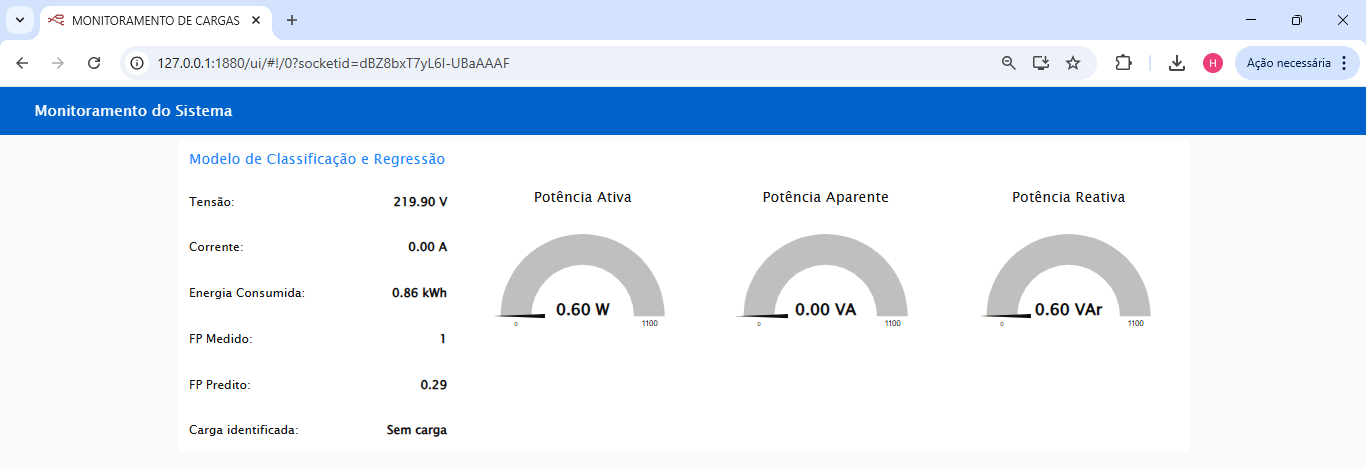
\includegraphics[width=1\textwidth]{Figuras/tela_sem_carga.png}
    \fonte{\me{2026}}
    \label{fig:painel_sem_carga}
\end{figure}

\begin{figure}[h]
    \centering
    \caption{Painel de monitoramento Node-RED para carga capacitiva.}
    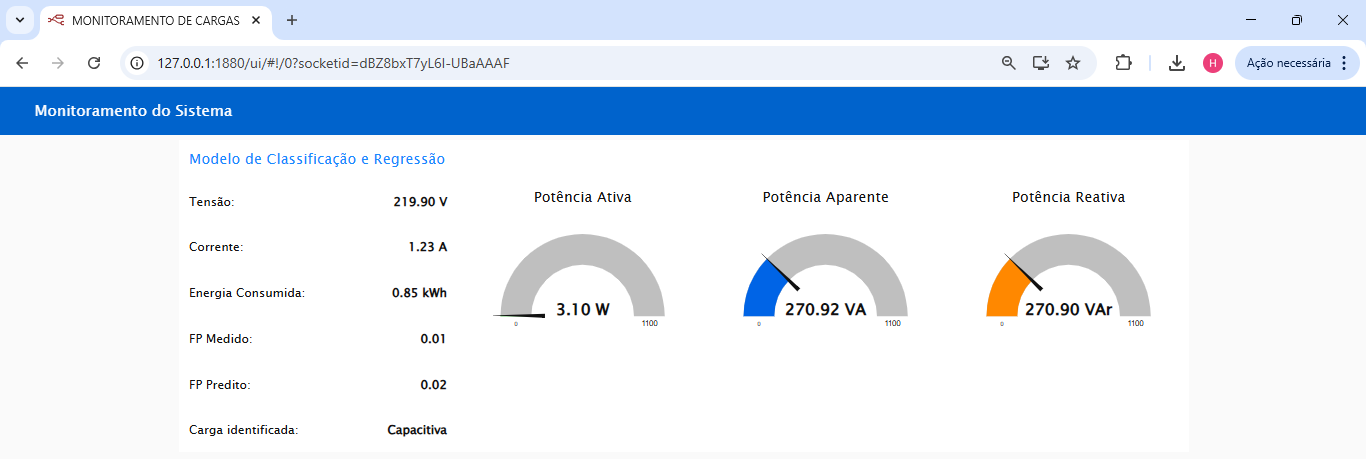
\includegraphics[width=1\textwidth]{Figuras/tela_carga_capacitiva.png}
    \fonte{\me{2026}}
    \label{fig:painel_capacitiva}
\end{figure}

\begin{figure}[h]
    \centering
    \caption{Painel de monitoramento Node-RED para carga indutiva.}
    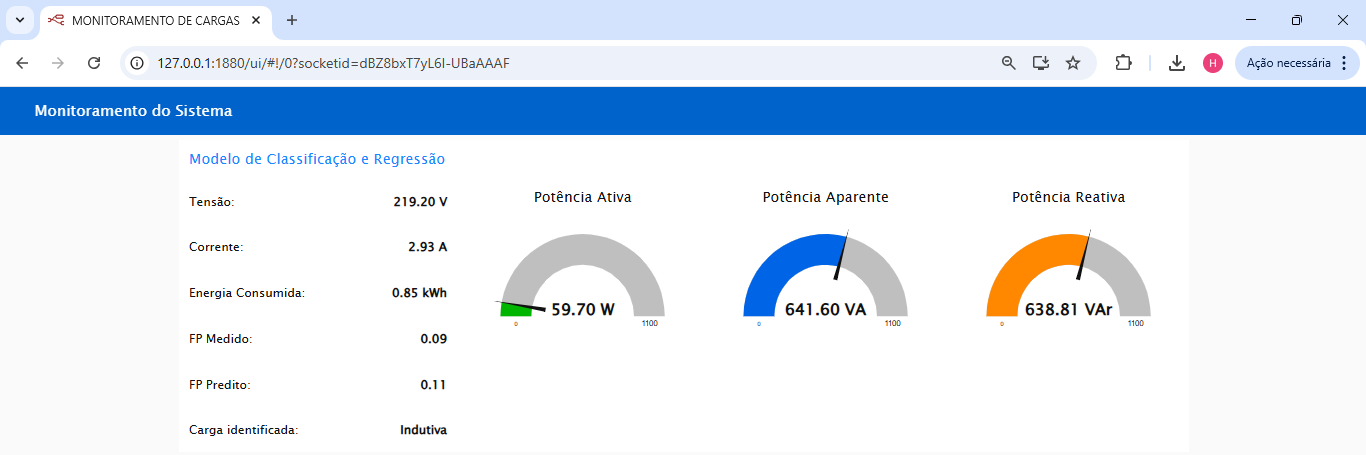
\includegraphics[width=1\textwidth]{Figuras/tela_carga_indutiva.png}
    \fonte{\me{2026}}
    \label{fig:painel_indutiva}
\end{figure}

\begin{figure}[h]
    \centering
    \caption{Painel de monitoramento Node-RED para carga resistiva.}
    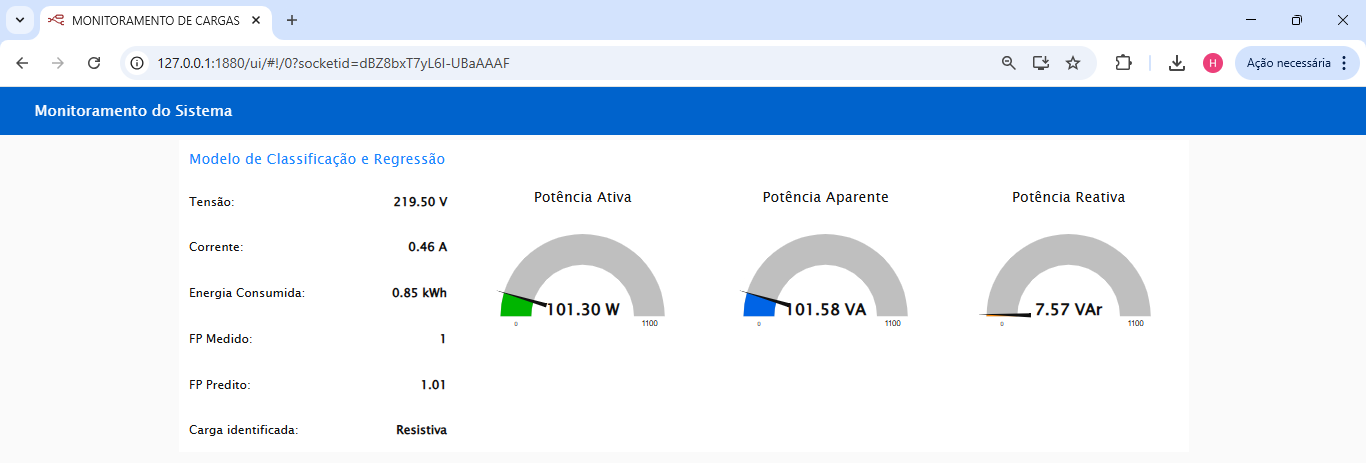
\includegraphics[width=1\textwidth]{Figuras/tela_carga_resistiva.png}
    \fonte{\me{2026}}
    \label{fig:painel_resistiva}
\end{figure}

\begin{figure}[h]
    \centering
    \caption{Painel de monitoramento Node-RED para motor.}
    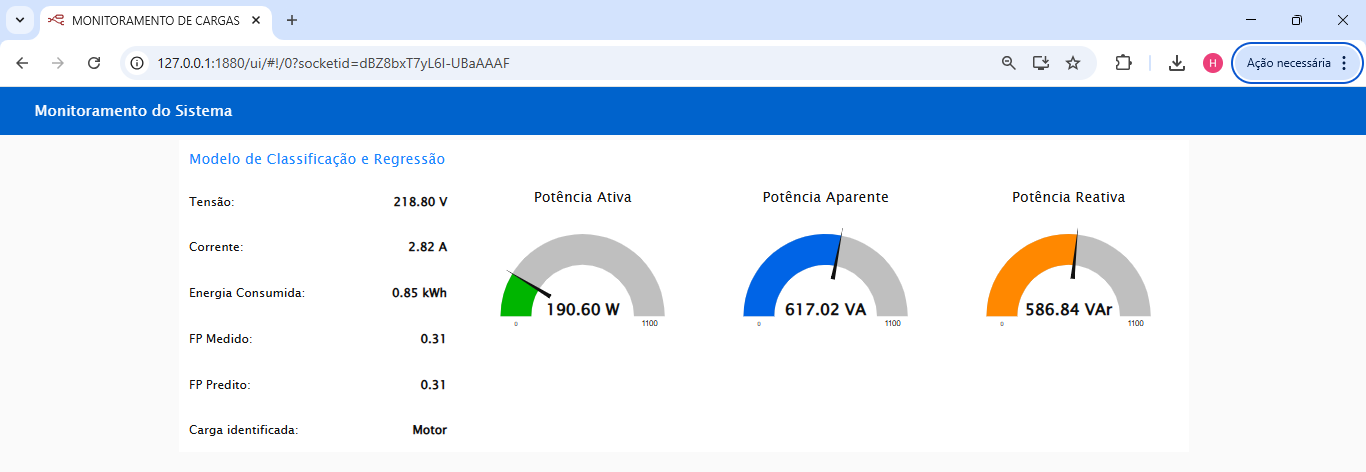
\includegraphics[width=1\textwidth]{Figuras/tela_carga_motor.png}
    \fonte{\me{2026}}
    \label{fig:painel_motor}
\end{figure}

\begin{figure}[h]
    \centering
    \caption{Painel de monitoramento Node-RED para carga resistiva + capacitiva.}
    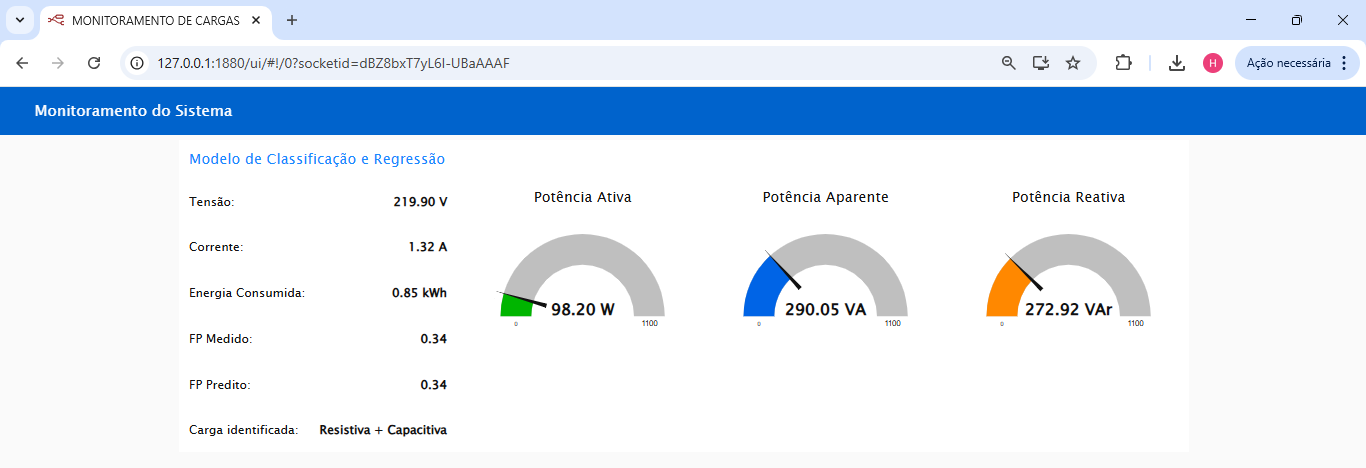
\includegraphics[width=1\textwidth]{Figuras/tela_carga_capacitiva_resisttiva.png}
    \fonte{\me{2026}}
    \label{fig:painel_res_cap}
\end{figure}

\begin{figure}[h]
    \centering
    \caption{Painel de monitoramento Node-RED para carga resistiva + indutiva.}
    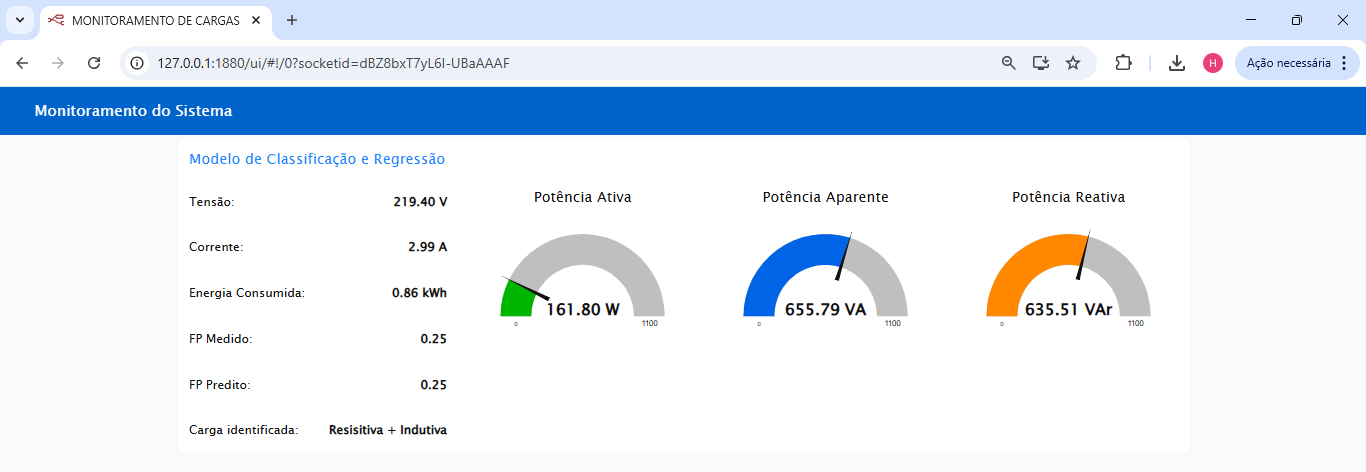
\includegraphics[width=1\textwidth]{Figuras/tela_carga_indutiva_resistiva.png}
    \fonte{\me{2026}}
    \label{fig:painel_res_ind}
\end{figure}

\begin{figure}[h]
    \centering
    \caption{Painel de monitoramento Node-RED para carga capacitiva + indutiva.}
    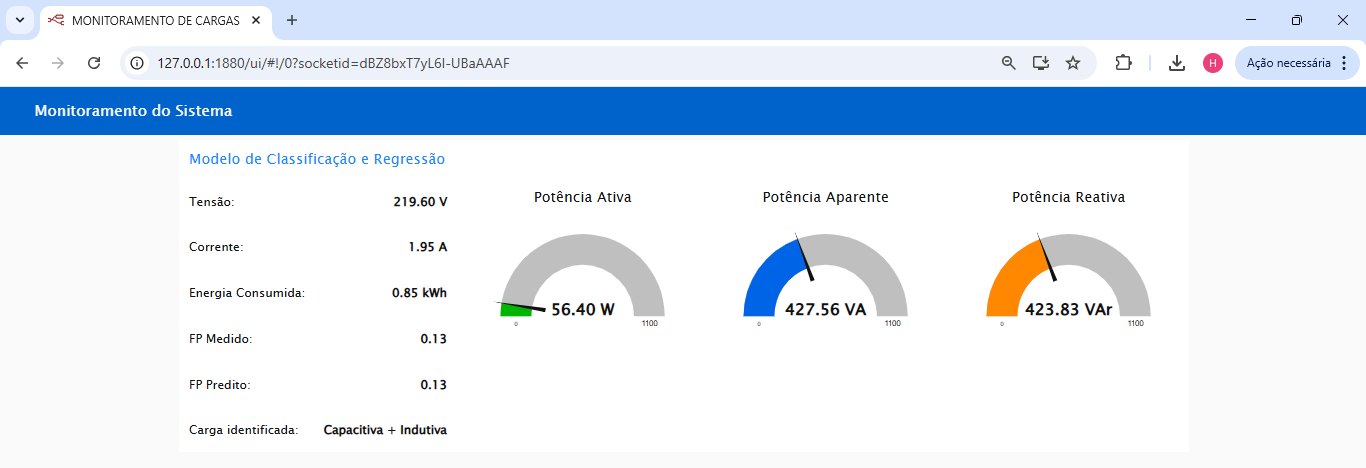
\includegraphics[width=1\textwidth]{Figuras/tela_carga_capacitiva_indutiva.png}
    \fonte{\me{2026}}
    \label{fig:painel_cap_ind}
\end{figure}

\clearpage
Apesar dos bons resultados obtidos, algumas limitações foram identificadas ao longo do desenvolvimento, para fins de considerações em melhorias futuras:
\begin{itemize}
    \item O sensor PZEM-004T apresentou pequenas variações nas medições em comparação com o medidor de referência, especialmente em condições de baixa carga;
    \item A base de dados experimental foi coletada em ambiente laboratorial controlado, podendo não refletir integralmente a complexidade de cenários reais;
    \item Os modelos foram treinados para oito classes de carga específicas (motor de indução, lâmpada incandescente, banco de capacitores de 15 $\mu$F, além de combinações entre eles), limitando sua aplicação a configurações similares e evidenciando a necessidade de expansão do horizonte de cargas;
    \item A estimativa do fator de potência na condição sem carga apresentou desvio devido a características intrínsecas do sensor.
\end{itemize}

% A Figura \ref{fig:painel_monitoramento_nodered} apresenta o painel de monitoramento desenvolvido no Node-RED, com as leituras do PZEM, o fator de potência estimado pelo modelo de regressão e a classe de carga identificada pelo modelo de classificação para cada cenário de carga testado.
% \begin{figure}[h]
%     \centering
%     \caption{Leituras do PZEM exibidas no painel de monitoramento Node-RED.}
    
%     % Linha 1
%     \subfigure[Sem carga]{
%         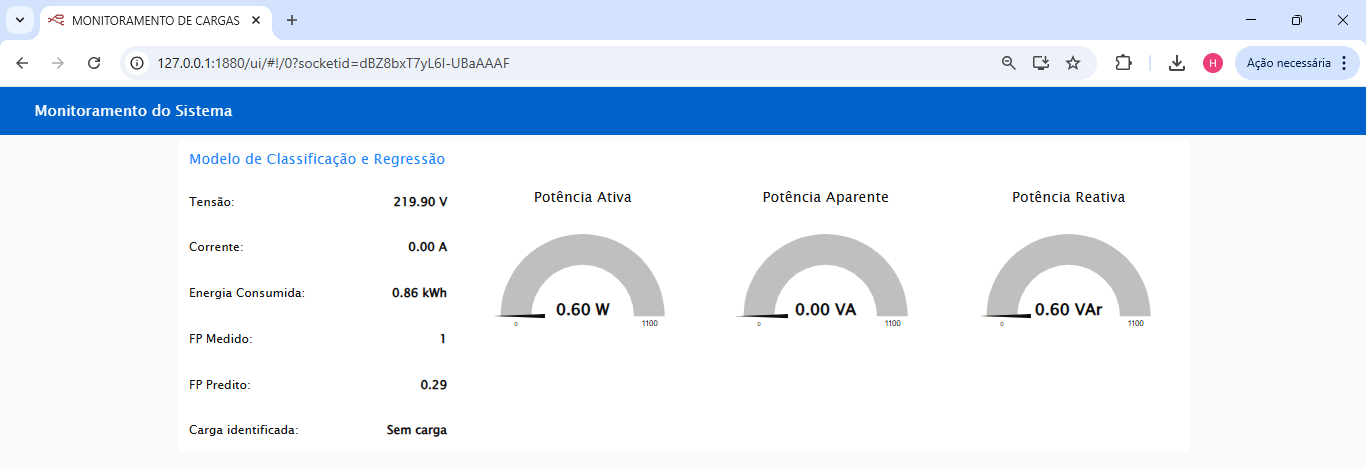
\includegraphics[width=0.48\textwidth]{Figuras/tela_sem_carga.png}
%     }
%     \hfill
%     \subfigure[Capacitiva]{
%         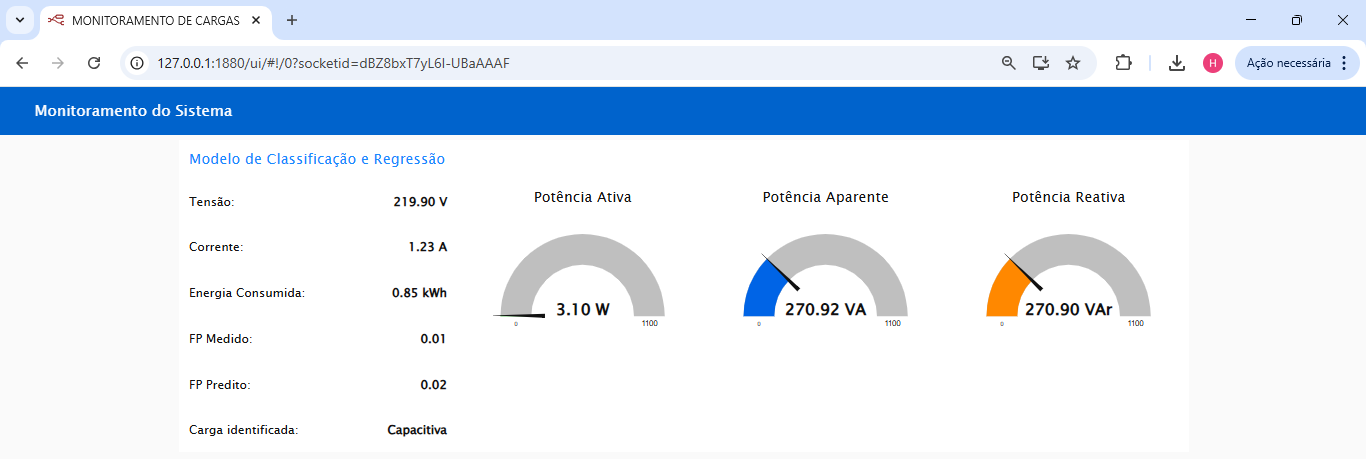
\includegraphics[width=0.48\textwidth]{Figuras/tela_carga_capacitiva.png}
%     }
    
%     \vspace{0.2cm}
    
%     % Linha 2
%     \subfigure[Indutiva]{
%         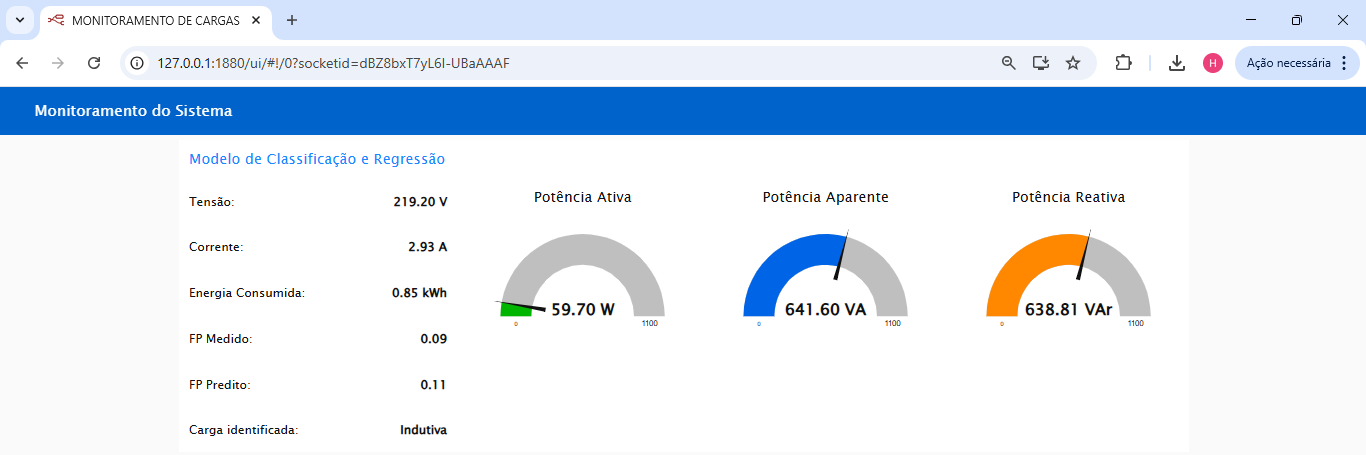
\includegraphics[width=0.48\textwidth]{Figuras/tela_carga_indutiva.png}
%     }
%     \hfill
%     \subfigure[Resistiva]{
%         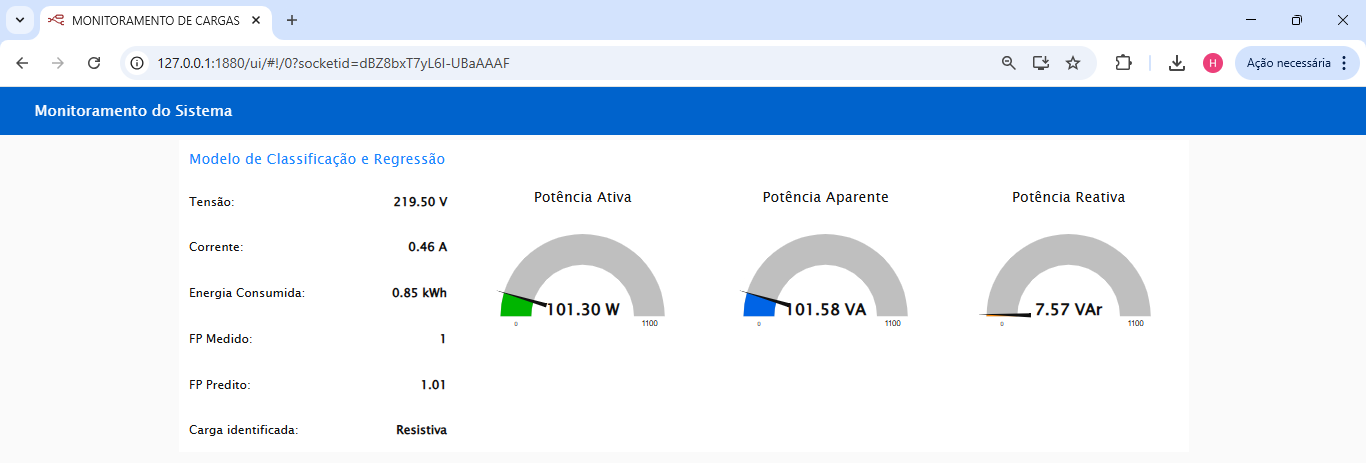
\includegraphics[width=0.48\textwidth]{Figuras/tela_carga_resistiva.png}
%     }
    
%     \vspace{0.2cm}
    
%     % Linha 3
%     \subfigure[Motor]{
%         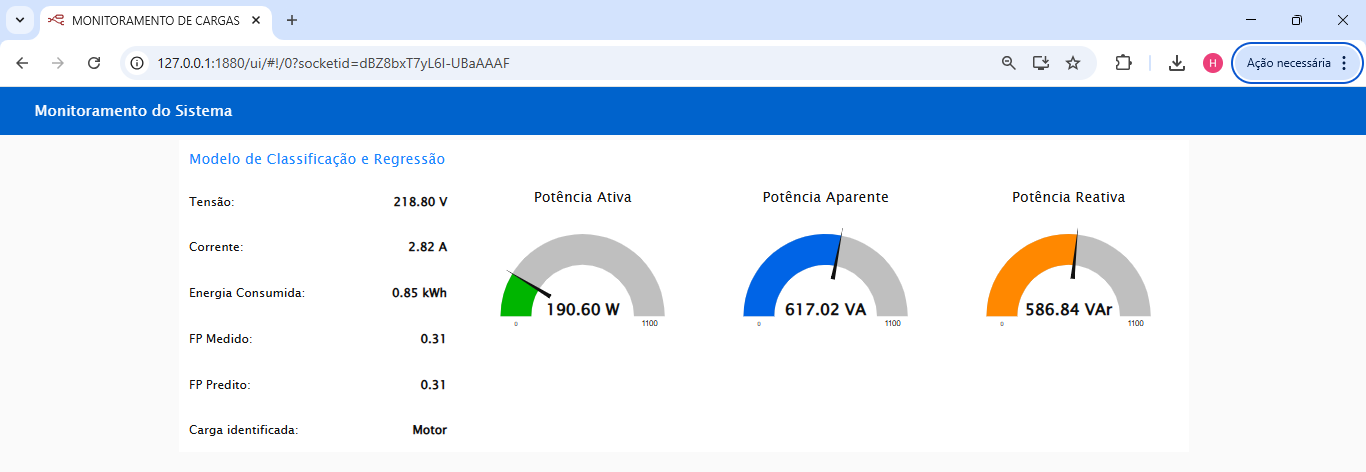
\includegraphics[width=0.48\textwidth]{Figuras/tela_carga_motor.png}
%     }
%     \hfill
%     \subfigure[Resistiva + Capacitiva]{
%         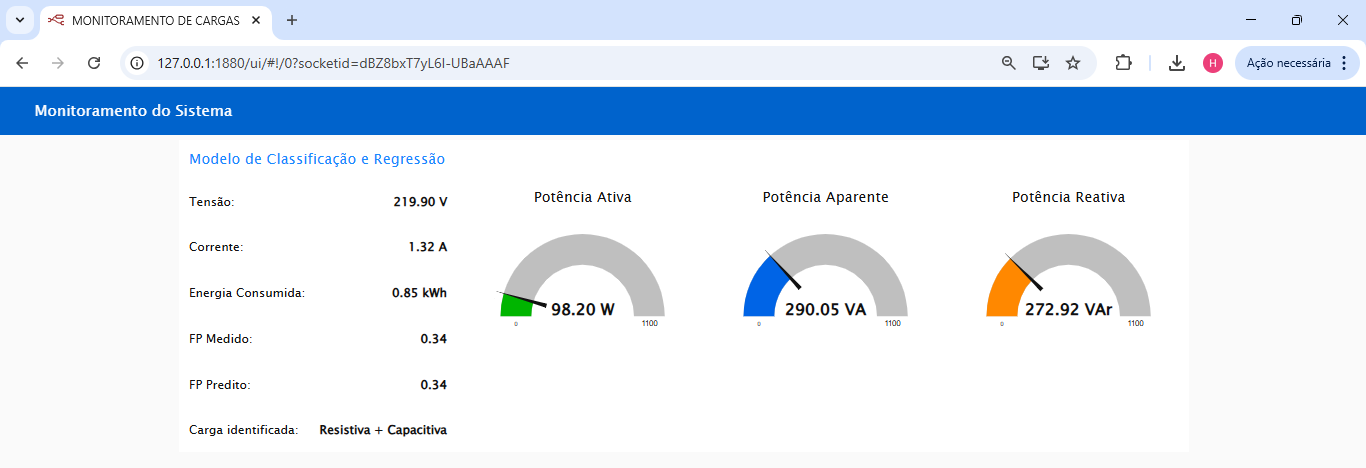
\includegraphics[width=0.48\textwidth]{Figuras/tela_carga_capacitiva_resisttiva.png}
%     }
    
%     \vspace{0.2cm}
    
%     % Linha 4
%     \subfigure[Resistiva + Indutiva]{
%         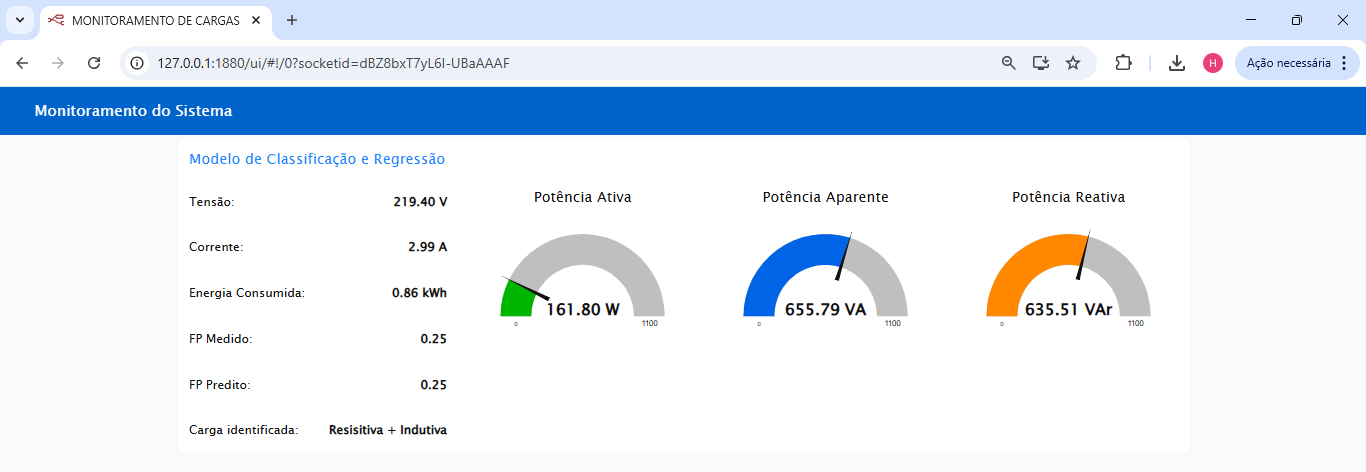
\includegraphics[width=0.48\textwidth]{Figuras/tela_carga_indutiva_resistiva.png}
%     }
%     \hfill
%     \subfigure[Capacitiva + Indutiva]{
%         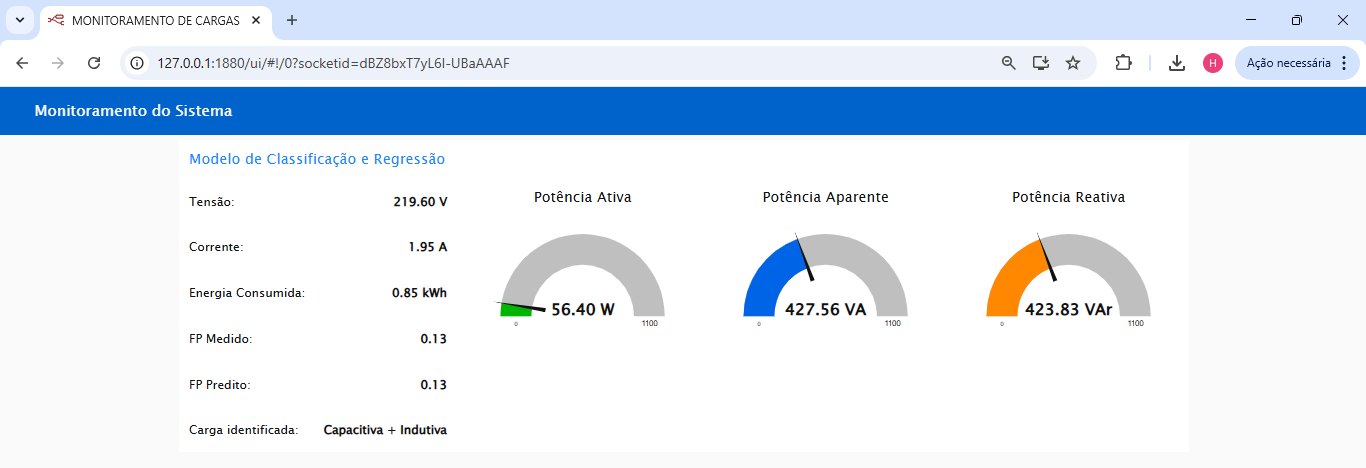
\includegraphics[width=0.48\textwidth]{Figuras/tela_carga_capacitiva_indutiva.png}
%     }
    
%     \fonte{\me{2026}}
%     \label{fig:painel_monitoramento_nodered}
% \end{figure}

% --------------------------------------------------------
% A análise exploratória da base residencial \textit{Individual Household Electric Power Consumption - UCI} teve como finalidade compreender o comportamento das grandezas elétricas e sua relação com o fator de potência (FP), com o objetivo de selecionar as variáveis de maior relevância para o treinamento dos modelos. 

% A base contempla medições realizadas entre os anos de 2006 e 2010, porém, para este estudo, foi selecionado um recorte correspondente a um ano completo de dados referente a 2010. O código desenvolvido e o acesso à base de dados dessa análise estão disponíveis no Apêndice \ref{apendice_análise_UCI}.

% Inicialmente, foi realizada uma análise da sazonalidade mensal do fator de potência médio, conforme ilustrado na Figura \ref{fig:fp_sazonalidade}. Os resultados permitem observar variações significativas ao longo do ano, indicando que o fator de potência sofre influência direta das mudanças no perfil de consumo e da combinação de cargas presentes no sistema elétrico ao longo das estações.

% \begin{figure}[!htbp] 
%     \centering
%     \caption{Análise de sazonalidade mensal do fator de potência.} 
%     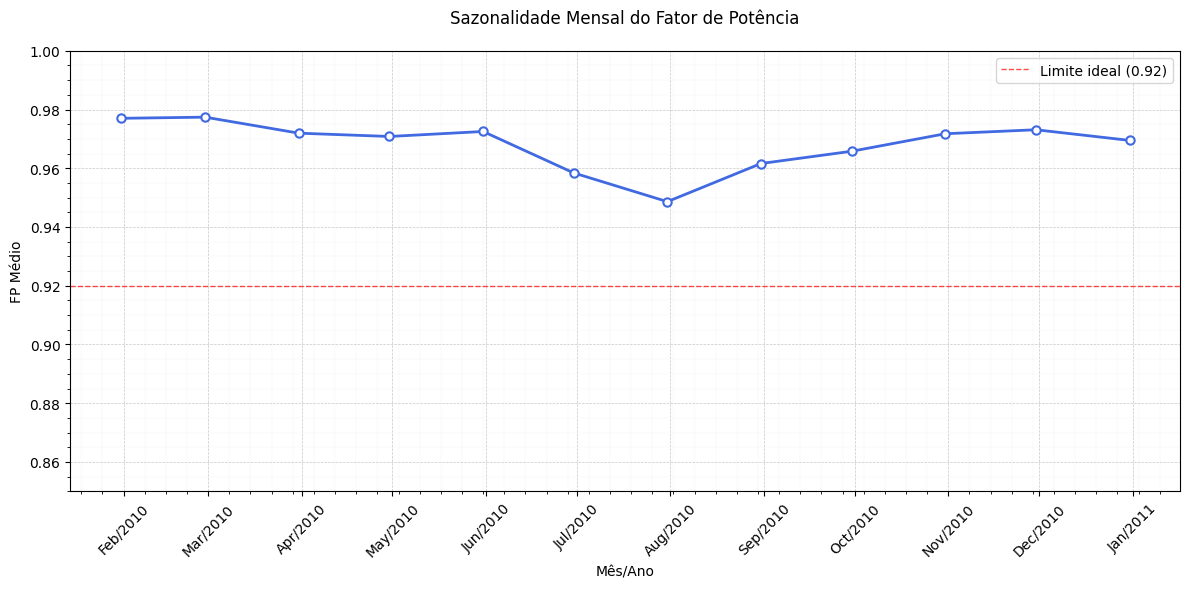
\includegraphics[width = 1\textwidth]{Figuras/sazonalidade mesal do fp.png} 
%     \fonte{\me{2026}} 
%     \label{fig:fp_sazonalidade} 
% \end{figure}

% Posteriormente, foi realizada a avaliação da correlação entre o fator de potência e as principais grandezas elétricas disponíveis na base de dados, incluindo potência ativa média global, potência reativa, tensão e intensidade de corrente média global. A matriz de correlação apresentada na Figura \ref{fig:correlacao_variaveis} mostra que o FP tem correlação negativa mais expressiva com a potência reativa ($r \approx -0{,}47$) e positiva fraca com potência ativa ($r \approx 0{,}40$). Embora as correlações entre o fator de potência, corrente e potência aparente sejam moderadas ($r \approx 0{,}38$), a corrente apresenta forte correlação com a potência ativa ($r \approx 1$) e com a potência aparente ($r \approx 1$), evidenciando a relação esperada entre essas grandezas. Por outro lado, a tensão apresentou correlação com o fator de potência praticamente nula ($r \approx 0{,}13$), o que indica que essa grandeza, isoladamente, não é um bom preditor do FP. Por esse motivo, não foi incluída como variável de entrada no treinamento dos modelos.

% \begin{figure}[!htbp] 
%     \centering
%     \caption{Matriz de correlação das variáveis elétricas.} 
%     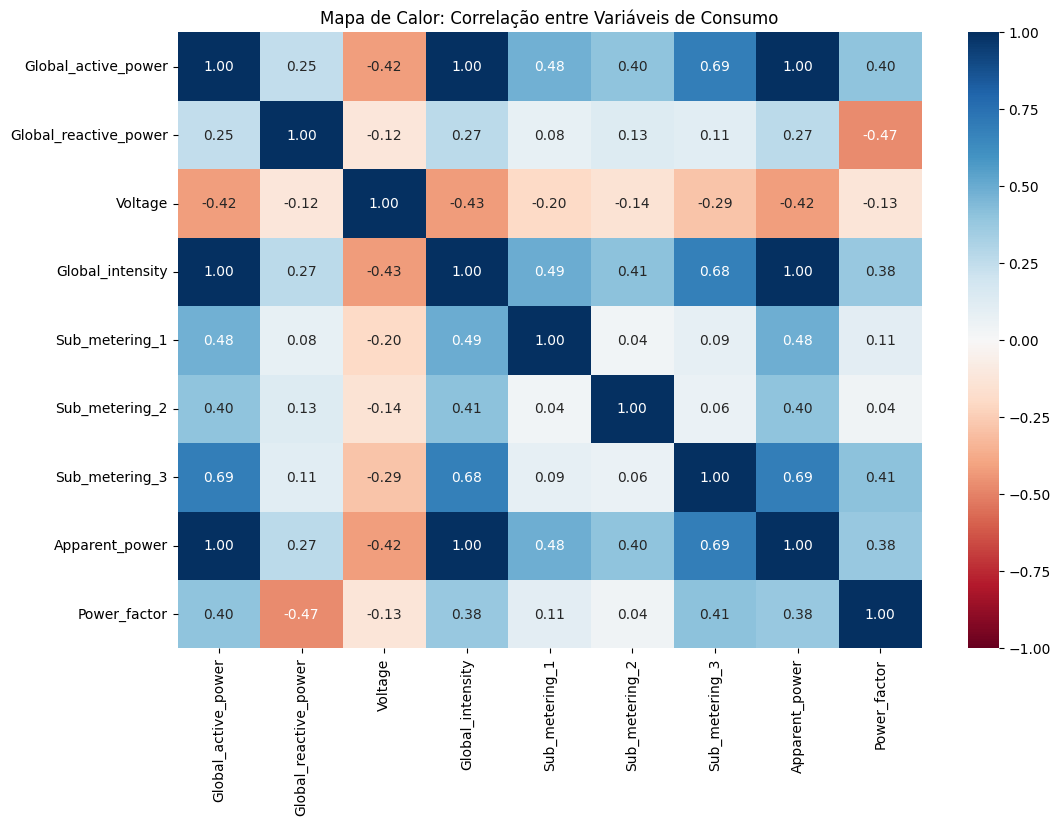
\includegraphics[width = 1\textwidth]{Figuras/mapa de correlação.png} 
%     \fonte{\me{2026}} 
%     \label{fig:correlacao_variaveis} 
% \end{figure}

% A análise evidenciou que o fator de potência apresenta relação significativa com as variáveis associadas às potências ativa, reativa, aparente e intensidade de corrente, conforme detalhado na Figura \ref{fig:graficos_relacao_fp}. Tal comportamento é esperado do ponto de vista físico, uma vez que o fator de potência está diretamente relacionado à relação entre potência ativa e aparente em sistemas elétricos, conforme Equação \eqref{eq:fp}. Dessa forma, variações nas potências e na corrente de consumo impactam diretamente o valor do fator de potência observado.

% Além disso, foram investigados os períodos de ocorrência dos menores valores de fator de potência ao longo da série temporal, buscando identificar possíveis padrões associados a mudanças no perfil de consumo. Para essa análise, foram considerados os 1\% menores valores de fator de potência da base de dados, correspondendo a valores iguais ou inferiores a 0,8057. Nesse subconjunto, observou-se um valor médio de 0,7829, com mínimo de 0,6175 e máximo de 0,8057, conforme Figura \ref{fig:resumo_estatistico_menores_FP}, caracterizando as condições mais críticas de operação em termos de fator de potência.

% \begin{figure}[!htbp] 
%     \centering
%     \caption{Resumo estatístico dos menores FPs.} 
%     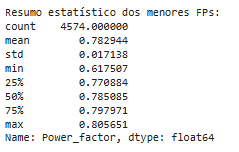
\includegraphics{Figuras/Resumo estatístico dos menores FPs.png} 
%     \fonte{\me{2026}} 
%     \label{fig:resumo_estatistico_menores_FP} 
% \end{figure}

% A distribuição temporal dessas ocorrências revelou um padrão horário bem definido. Conforme ilustrado na Figura \ref{fig:distribuicao_menores_fp}, a maior concentração de valores críticos ocorre durante o período da madrugada, com pico de ocorrências às 4h (377 registros). Esse comportamento sugere que os menores valores de fator de potência tendem a ocorrer em períodos de menor demanda elétrica global, quando a participação relativa de cargas com características reativas se torna mais significativa. Esse padrão pode estar associado ao funcionamento de determinados equipamentos operando em regime contínuo durante a madrugada, como motores de pequena potência e sistemas de refrigeração.

% \begin{figure}[!htbp] 
%     \centering
%     \caption{Distribuição horária das ocorrências dos menores valores de fator de potência.} 
%     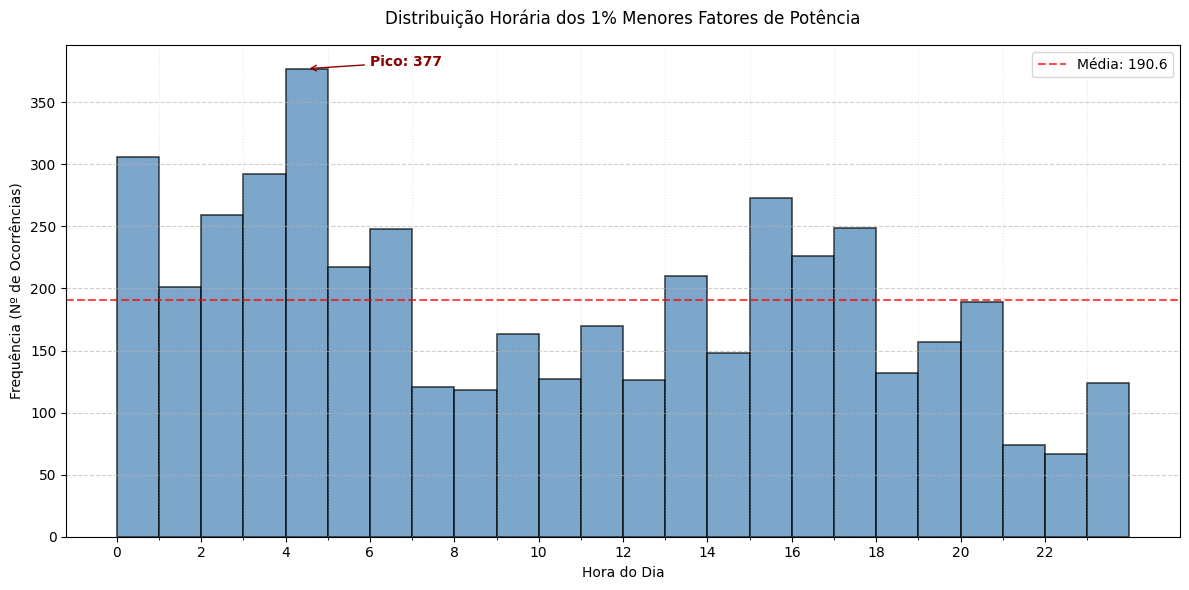
\includegraphics[width=1\textwidth]{Figuras/distribuicao menores fp.png} 
%     \fonte{\me{2026}} 
%     \label{fig:distribuicao_menores_fp} 
% \end{figure} 

% \begin{figure}[h]
%     \centering
%     \caption{Relações entre grandezas elétricas e o fator de potência}
%     \subfigure[Relação P x FP.]{
%         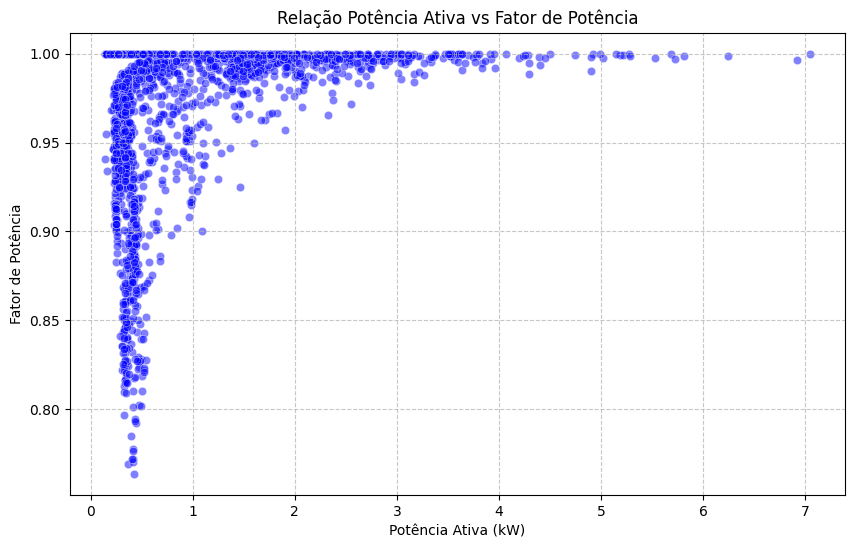
\includegraphics[width=0.75\textwidth]{Figuras/grafico de relação P VS fp.png}
%     }
%     \hfill % Adiciona espaço entre as imagens
%     \subfigure[Relação Q x FP.]{
%         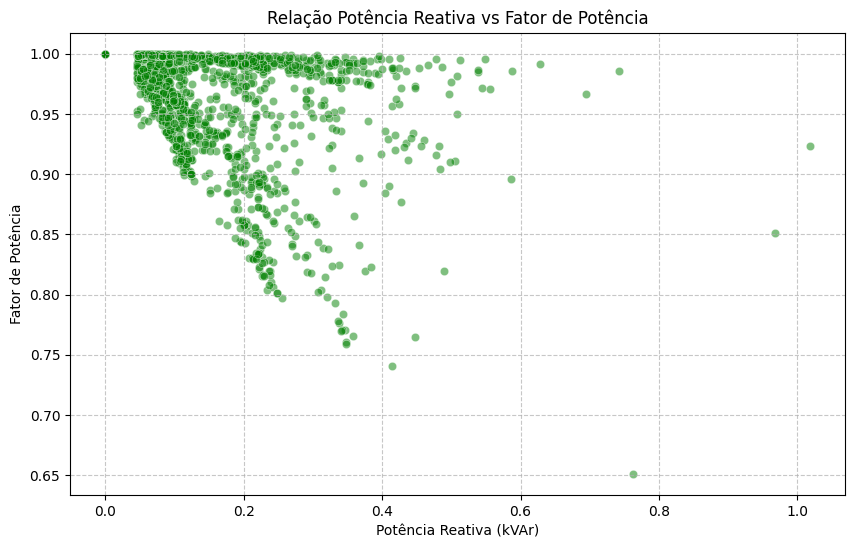
\includegraphics[width=0.75\textwidth]{Figuras/grafico de relação Q VS fp.png}
%     }
%     \hfill
%     \subfigure[Relação I x FP.]{
%         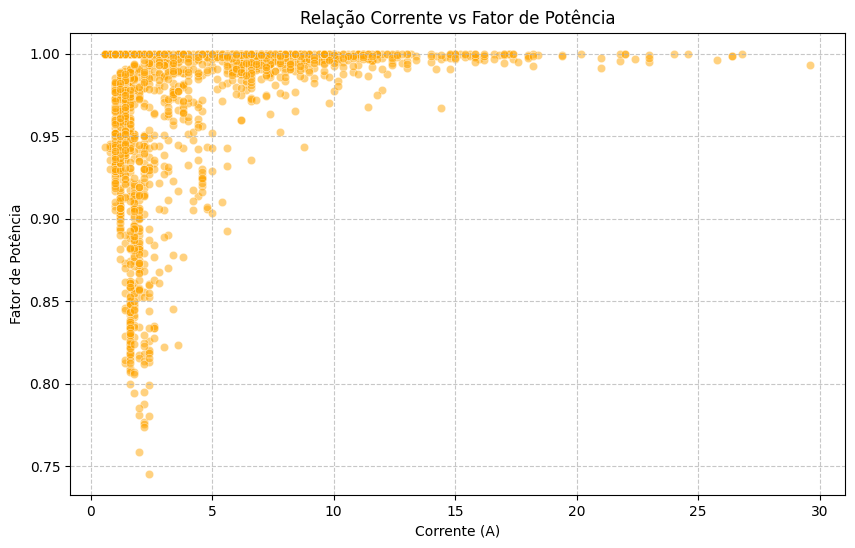
\includegraphics[width=0.75\textwidth]{Figuras/grafico de relação I VS fp.png}
%     }
%     \fonte{\me{2026}} 
%     \label{fig:graficos_relacao_fp}
% \end{figure}
